\documentclass[aspectratio=169, 10pt]{beamer}

% ── Theme & Colors ──
\usetheme{Madrid}
\usecolortheme{whale}
\setbeamertemplate{navigation symbols}{}
\setbeamertemplate{footline}[frame number]

% ── Packages ──
\usepackage[utf8]{inputenc}
\usepackage{graphicx}
\usepackage{booktabs}
\usepackage{amsmath}
\usepackage{tikz}
\usetikzlibrary{arrows.meta, positioning, shapes.geometric, fit, calc}
\usepackage{multicol}
\usepackage{xcolor}
\usepackage{hyperref}
\usepackage{textcomp}
\graphicspath{{images/}}
\usepackage{multirow}
\usepackage{colortbl}
\usepackage{array}

\definecolor{okgreen}{RGB}{50,150,50}
\definecolor{warnred}{RGB}{200,50,50}
\definecolor{infobl}{RGB}{40,100,180}
\definecolor{lightyellow}{RGB}{255,255,220}
\definecolor{lightblue}{RGB}{220,235,255}
\definecolor{lightgreen}{RGB}{220,255,220}
\definecolor{lightred}{RGB}{255,225,225}
\definecolor{boxblue}{RGB}{0,80,160}
\definecolor{boxorange}{RGB}{200,100,0}
\definecolor{boxgreen}{RGB}{0,130,60}
\definecolor{boxpurple}{RGB}{120,50,160}

% ── TikZ Styles (must be in preamble for beamer compatibility) ──
\tikzset{
    % Problem Statement
    catbox/.style={rectangle, rounded corners=3pt, draw=#1, fill=#1!10,
                text width=3.6cm, minimum height=0.7cm, align=center,
                font=\scriptsize\bfseries},
    % Overview pipeline
    pipebox/.style={rectangle, rounded corners=4pt, draw=#1, fill=#1!8,
                minimum width=4.2cm, minimum height=1.4cm, align=center, font=\small},
    pipelbl/.style={font=\scriptsize, text=gray!70},
    % Weather pipeline
    wnode/.style={rectangle, rounded corners=3pt, draw=boxblue, fill=boxblue!8,
                 minimum width=2.2cm, minimum height=0.85cm, align=center, font=\footnotesize},
    wssim/.style={rectangle, rounded corners=3pt, draw=warnred, fill=warnred!8,
                 minimum width=2.2cm, minimum height=0.85cm, align=center, font=\footnotesize},
    warrow/.style={-{Stealth[length=2.5mm]}, thick, boxblue!60},
    wnote/.style={font=\tiny, text=gray!80},
    % Day2Night pipeline
    dnode/.style={rectangle, rounded corners=3pt, draw=boxorange, fill=boxorange!8,
                 minimum width=3.5cm, minimum height=0.8cm, align=center, font=\footnotesize},
    darrow/.style={-{Stealth[length=2.5mm]}, thick, boxorange!60},
    % Fog pipeline
    fnode/.style={rectangle, rounded corners=3pt, draw=boxpurple, fill=boxpurple!8,
                 minimum width=2.8cm, minimum height=0.8cm, align=center, font=\footnotesize},
    farrow/.style={-{Stealth[length=2.5mm]}, thick, boxpurple!60},
    % Diffusion weather pipeline
    dwnode/.style={rectangle, rounded corners=3pt, draw=teal, fill=teal!8,
                  minimum width=2.8cm, minimum height=0.8cm, align=center, font=\footnotesize},
    dwarrow/.style={-{Stealth[length=2.5mm]}, thick, teal!60},
    % Outpainting pipeline
    onode/.style={rectangle, rounded corners=3pt, draw=boxgreen, fill=boxgreen!8,
                 minimum width=3.8cm, minimum height=0.7cm, align=center, font=\footnotesize},
    oarrow/.style={-{Stealth[length=2.5mm]}, thick, boxgreen!60},
    % Repo structure
    rdir/.style={rectangle, rounded corners=2pt, draw=#1, fill=#1!8,
                minimum width=2.8cm, minimum height=0.6cm, align=center,
                font=\footnotesize\ttfamily},
    rroot/.style={rectangle, rounded corners=4pt, draw=black, fill=gray!10,
                 minimum width=2.8cm, minimum height=0.65cm, align=center,
                 font=\footnotesize\bfseries\ttfamily},
    rarrow/.style={-{Stealth[length=2mm]}, thick, gray!50},
    rdesc/.style={font=\tiny, text=gray!80},
    % General
    garrow/.style={-{Stealth[length=3mm]}, thick, gray!70},
}

% ── Title ──
\title[ConSynth-X]{ConSynth-X: Benchmarking Construction CV\\Under Extreme Field Conditions}
\subtitle{Project Progress Report}
\author{Viet Huy Duong \\ \texttt{vduong1@kent.edu}}
\institute{Kent State University}
\date{April 8, 2026}

\begin{document}

% ════════════════════════════════════════
\begin{frame}
\titlepage
\end{frame}

% ════════════════════════════════════════
\begin{frame}{Outline}
\tableofcontents
\end{frame}

% ════════════════════════════════════════
\section{Problem \& Motivation}
% ════════════════════════════════════════

\begin{frame}{Problem Statement}
\begin{columns}[T]
\begin{column}{0.55\textwidth}
\textbf{Goal:} Evaluate how robust construction computer vision models are under extreme field conditions.

\vspace{0.5em}
\textbf{Why this matters:}
\begin{itemize}
    \item Construction sites face rain, snow, fog, low light, glare
    \item Models trained on clean data fail in the field
    \item No standardized benchmark for these conditions
\end{itemize}

\vspace{0.5em}
\textbf{ConSynth-X provides:}
\begin{enumerate}
    \item Synthetic augmentation pipelines (5 methods)
    \item Multi-label taxonomy of 40+ conditions
    \item VLM benchmarking framework (11 models)
    \item Image quality evaluation (FID, DINO structure)
\end{enumerate}
\end{column}
\begin{column}{0.42\textwidth}
\centering
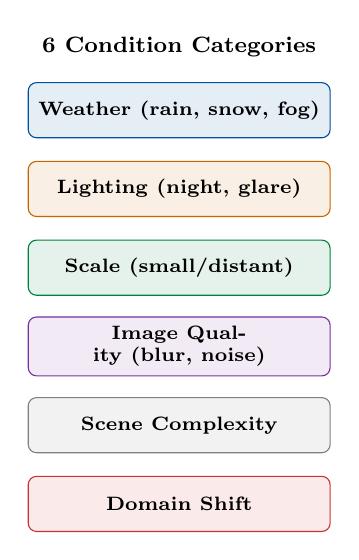
\begin{tikzpicture}
\node[catbox=boxblue]   (w) at (0,3)   {Weather (rain, snow, fog)};
\node[catbox=boxorange] (l) at (0,2)   {Lighting (night, glare)};
\node[catbox=boxgreen]  (s) at (0,1)   {Scale (small/distant)};
\node[catbox=boxpurple] (q) at (0,0)   {Image Quality (blur, noise)};
\node[catbox=gray]      (c) at (0,-1)  {Scene Complexity};
\node[catbox=warnred]   (d) at (0,-2)  {Domain Shift};

\node[font=\footnotesize\bfseries, above=0.2cm of w] {6 Condition Categories};
\end{tikzpicture}
\end{column}
\end{columns}
\end{frame}

% ════════════════════════════════════════
\section{Datasets}
% ════════════════════════════════════════

\begin{frame}{Base Datasets}
\begin{columns}[T]
\begin{column}{0.48\textwidth}
\textbf{\textcolor{boxblue}{ConstructionSite10k}}
\begin{itemize}
    \item Format: HuggingFace Arrow
    \item 3 classes: \texttt{excavator}, \texttt{rebar}, \texttt{worker\_with\_white\_hard\_hat}
    \item Test set: \textbf{3,004} images
    \item Rich annotations: bounding boxes + 4 safety rules + captions
\end{itemize}
\end{column}
\begin{column}{0.48\textwidth}
\textbf{\textcolor{boxorange}{SODA Dataset}}
\begin{itemize}
    \item Format: Pascal VOC (XML)
    \item \textbf{15} object classes
    \item Total: \textbf{19,846} images
    \item Standard VOC train/val/test splits
\end{itemize}
\end{column}
\end{columns}

\vspace{0.4em}
\centering
{\small
\begin{tabular}{lccc}
\toprule
\textbf{Condition} & \textbf{Method} & \textbf{Constr. Site} & \textbf{SODA} \\
\midrule
Original        & Baseline              & 3,004  & 19,846 \\
Weather (style) & Neural Style Transfer & 10,266 & 47,169 \\
Weather (diff.) & InstructPix2Pix       & 10,382 & --     \\
Night           & img2img-turbo         & 3,004  & 19,846 \\
\rowcolor{lightblue}
Night Weather   & Night $\to$ IP2P + Physics & Pending & --  \\
Fog             & Koschmieder + DA V2   & 3,003  & --     \\
Small           & FLUX Outpainting      & 1,323  & 1,001  \\
\midrule
\textbf{Total} &                        & \textbf{30,982+} & \textbf{87,862} \\
\bottomrule
\end{tabular}
}
\end{frame}

% ════════════════════════════════════════
\section{Augmentation Pipelines}
% ════════════════════════════════════════

\begin{frame}{Overview of 5 Augmentation Pipelines}
\centering
\scalebox{0.78}{%
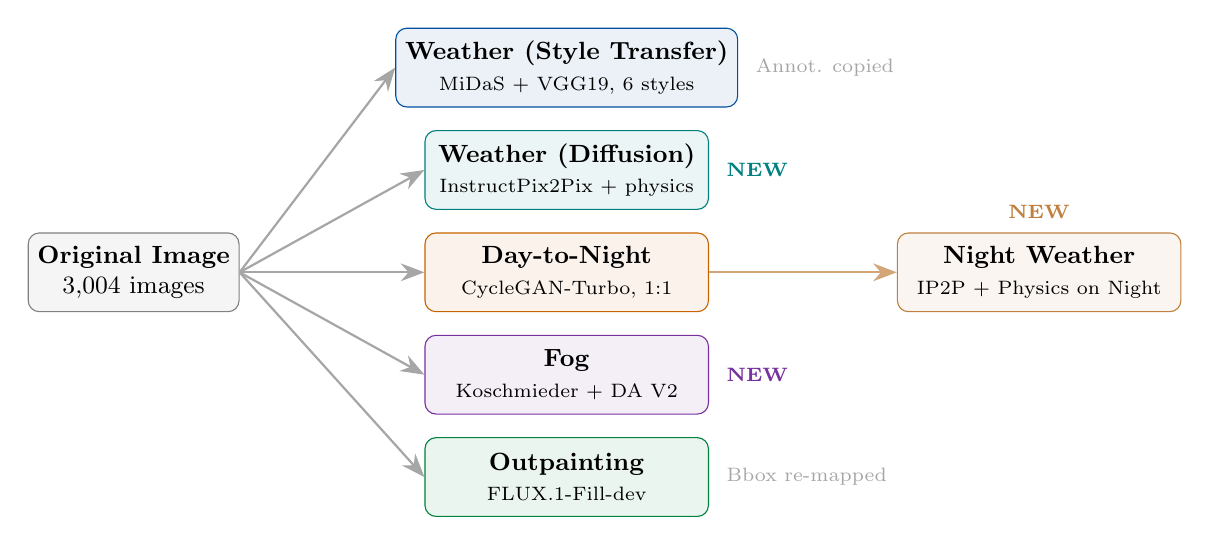
\begin{tikzpicture}
% Original
\node[pipebox=gray, minimum width=2.6cm, minimum height=1.0cm] (orig) at (0,0) {\textbf{Original Image}\\3,004 images};

% Weather (old)
\node[pipebox=boxblue, minimum width=3.6cm, minimum height=1.0cm] (weather) at (5.5,2.6) {
    \textbf{Weather (Style Transfer)}\\
    {\scriptsize MiDaS + VGG19, 6 styles}
};

% Weather (new - diffusion)
\node[pipebox=teal, minimum width=3.6cm, minimum height=1.0cm] (diffweather) at (5.5,1.3) {
    \textbf{Weather (Diffusion)}\\
    {\scriptsize InstructPix2Pix + physics}
};

% Night
\node[pipebox=boxorange, minimum width=3.6cm, minimum height=1.0cm] (night) at (5.5,0) {
    \textbf{Day-to-Night}\\
    {\scriptsize CycleGAN-Turbo, 1:1}
};

% Fog
\node[pipebox=boxpurple, minimum width=3.6cm, minimum height=1.0cm] (fog) at (5.5,-1.3) {
    \textbf{Fog}\\
    {\scriptsize Koschmieder + DA V2}
};

% Night Weather (compound)
\node[pipebox=brown, minimum width=3.6cm, minimum height=1.0cm] (nightweather) at (11.5,0) {
    \textbf{Night Weather}\\
    {\scriptsize IP2P + Physics on Night}
};

% Small
\node[pipebox=boxgreen, minimum width=3.6cm, minimum height=1.0cm] (small) at (5.5,-2.6) {
    \textbf{Outpainting}\\
    {\scriptsize FLUX.1-Fill-dev}
};

% Arrows
\draw[garrow] (orig.east) -- (weather.west);
\draw[garrow] (orig.east) -- (diffweather.west);
\draw[garrow] (orig.east) -- (night.west);
\draw[garrow] (orig.east) -- (fog.west);
\draw[garrow] (orig.east) -- (small.west);

% Night → Night Weather
\draw[garrow, brown!70] (night.east) -- (nightweather.west);

% Annotations
\node[pipelbl, right=0.1cm of weather.east] {Annot. copied};
\node[pipelbl, right=0.1cm of diffweather.east] {\textcolor{teal}{\textbf{NEW}}};
\node[pipelbl, right=0.1cm of fog.east]     {\textcolor{boxpurple}{\textbf{NEW}}};
\node[pipelbl, right=0.1cm of small.east]   {Bbox re-mapped};
\node[pipelbl, above=0.05cm of nightweather.north] {\textcolor{brown}{\textbf{NEW}}};

\end{tikzpicture}}%
\end{frame}

% ────────────────────────────────────────
\begin{frame}{Weather Augmentation Pipeline}
\centering
\resizebox{\textwidth}{!}{%
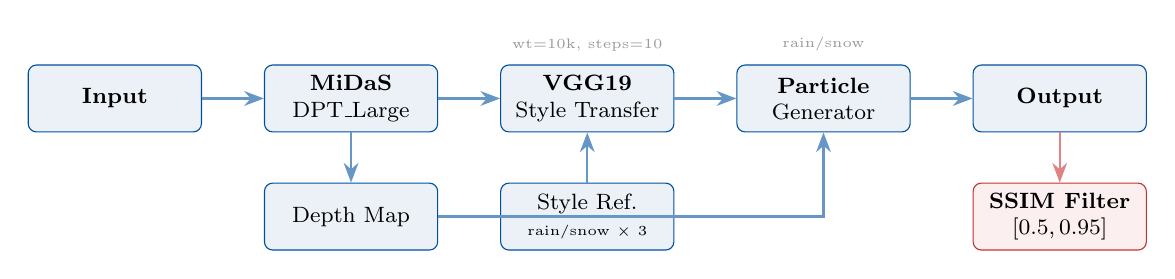
\begin{tikzpicture}
\node[wnode] (input) at (0,0)    {\textbf{Input}};
\node[wnode] (midas) at (3,0)    {\textbf{MiDaS}\\DPT\_Large};
\node[wnode] (depth) at (3,-1.5) {Depth Map};
\node[wnode] (vgg)   at (6,0)    {\textbf{VGG19}\\Style Transfer};
\node[wnode] (style) at (6,-1.5) {Style Ref.\\{\tiny rain/snow $\times$ 3}};
\node[wnode] (part)  at (9,0)    {\textbf{Particle}\\Generator};
\node[wnode] (out)   at (12,0)   {\textbf{Output}};
\node[wssim] (ssim) at (12,-1.5) {\textbf{SSIM Filter}\\$[0.5, 0.95]$};

\draw[warrow] (input) -- (midas);
\draw[warrow] (midas) -- (depth);
\draw[warrow] (midas) -- (vgg);
\draw[warrow] (depth) -| (part);
\draw[warrow] (style) -- (vgg);
\draw[warrow] (vgg) -- (part);
\draw[warrow] (part) -- (out);
\draw[warrow, draw=warnred!60] (out) -- (ssim);

\node[wnote, above=0.05cm of vgg] {wt=10k, steps=10};
\node[wnote, above=0.05cm of part] {rain/snow};
\end{tikzpicture}}%

\vspace{0.6em}
\begin{columns}[T]
\begin{column}{0.48\textwidth}
\centering
{\footnotesize \textbf{Construction Site} (3,004 original)}\\[0.3em]
\begin{tabular}{lc}
\toprule
\textbf{Style} & \textbf{After Filter} \\
\midrule
rain\_0 / rain\_1 / rain\_2 & 2,211 / 1,243 / 1,208 \\
snow\_0 / snow\_1 / snow\_2 & 2,159 / 1,649 / 1,796 \\
\midrule
\textbf{Total} & \textbf{10,266} \\
\bottomrule
\end{tabular}
\end{column}
\begin{column}{0.48\textwidth}
\centering
{\footnotesize \textbf{SODA} (19,846 original)}\\[0.3em]
\begin{tabular}{lc}
\toprule
\textbf{Style} & \textbf{After Filter} \\
\midrule
rain\_0 / rain\_1 / rain\_2 & 8,392 / 8,059 / 9,541 \\
snow\_0 / snow\_1 / snow\_2 & 9,818 / 7,485 / 3,874 \\
\midrule
\textbf{Total} & \textbf{47,169} \\
\bottomrule
\end{tabular}
\end{column}
\end{columns}
\end{frame}

% ────────────────────────────────────────
\begin{frame}{NEW: Diffusion-Based Rain/Snow (InstructPix2Pix)}
\begin{columns}[T]
\begin{column}{0.52\textwidth}
\textbf{Model:} InstructPix2Pix (\texttt{timbrooks/instruct-pix2pix})

\vspace{0.3em}
\textbf{Why IP2P?} Replaces neural style transfer with direct text-guided image editing while preserving scene structure.

\vspace{0.3em}
\textbf{Hybrid approach:} IP2P atmosphere + physics overlay
\begin{itemize}
    \item IP2P: dark sky, wet ground, frost, snow cover
    \item Physics: rain streaks (3 layers, 2800--5200) + fog overlay
    \item Snowflakes: 3 layers, 2100--3300, screen blend
\end{itemize}

\vspace{0.3em}
\textbf{Key parameters:}

{\scriptsize
\begin{tabular}{lcc}
\toprule
 & \textbf{Rain} & \textbf{Snow} \\
\midrule
\texttt{image\_guidance} & 1.5 & 1.5 \\
\texttt{guidance\_scale} & 10.0 & 8.0 \\
\texttt{steps} & 30 & 30 \\
\bottomrule
\end{tabular}
}
\end{column}
\begin{column}{0.45\textwidth}
\centering
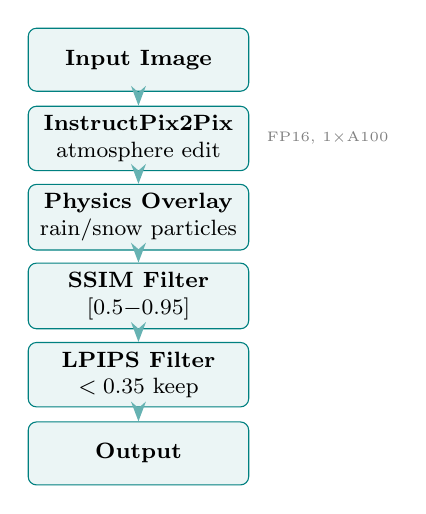
\begin{tikzpicture}
\node[dwnode] (in)      at (0,4)   {\textbf{Input Image}};
\node[dwnode] (ip2p)    at (0,3)   {\textbf{InstructPix2Pix}\\atmosphere edit};
\node[dwnode] (phys)    at (0,2)   {\textbf{Physics Overlay}\\rain/snow particles};
\node[dwnode] (ssim)    at (0,1)   {\textbf{SSIM Filter}\\$[0.5{-}0.95]$};
\node[dwnode] (lpips)   at (0,0)   {\textbf{LPIPS Filter}\\$< 0.35$ keep};
\node[dwnode] (out)     at (0,-1)  {\textbf{Output}};

\draw[dwarrow] (in) -- (ip2p);
\draw[dwarrow] (ip2p) -- (phys);
\draw[dwarrow] (phys) -- (ssim);
\draw[dwarrow] (ssim) -- (lpips);
\draw[dwarrow] (lpips) -- (out);

\node[font=\tiny, text=gray, right=0.1cm of ip2p] {FP16, 1$\times$A100};
\end{tikzpicture}

\vspace{0.3em}
{\scriptsize \textbf{Post-filter:} SSIM rejects unchanged/corrupted; LPIPS rejects structural loss $\geq 0.35$.}
\end{column}
\end{columns}
\end{frame}

% ────────────────────────────────────────
\begin{frame}{Weather Augmentation: Visual Comparison}
\centering
\includegraphics[width=\textwidth]{fig1_comparison_grid.png}

\vspace{0.3em}
{\scriptsize Original $\to$ Style Transfer (VGG19+MiDaS) $\to$ IP2P Diffusion (+ physics overlay).\\
Style transfer produces color/texture shifts; IP2P generates more physically consistent atmospheric effects.}
\end{frame}

% ────────────────────────────────────────
\begin{frame}{Night Weather Augmentation (IP2P + Physics)}
\begin{columns}[T]
\begin{column}{0.38\textwidth}
{\small \textbf{Pipeline:} Night $\rightarrow$ IP2P $\rightarrow$ Physics Particles}

\vspace{0.2em}
{\scriptsize Compound conditions (rain+night, snow+night) are common on real sites but absent from training data.}

\vspace{0.2em}
{\scriptsize
\begin{enumerate}\setlength{\itemsep}{0pt}
    \item Start from \textbf{CycleGAN night} image
    \item IP2P edits atmosphere (night prompts)
    \item Physics overlay: rain streaks / snowflakes
    \item SSIM/LPIPS filter (vs.\ \textit{original})
\end{enumerate}}

\vspace{0.1em}
{\tiny
\begin{tabular}{lcc}
\toprule
\textbf{Param} & \textbf{Rain} & \textbf{Snow} \\
\midrule
guidance\_scale & 10.0 & 8.0 \\
img\_guidance   & 1.5  & 1.5  \\
steps           & 30   & 30   \\
SSIM range      & {[}0.6, 0.95{]} & {[}0.5, 0.95{]} \\
LPIPS           & $<$0.35 & -- \\
\bottomrule
\end{tabular}
}

\vspace{0.1em}
\centering
\scalebox{0.7}{%
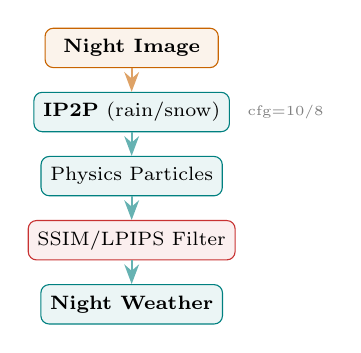
\begin{tikzpicture}[node distance=0.3cm]
\node[dnode, minimum width=2.2cm, minimum height=0.5cm, font=\scriptsize] (n)  {\textbf{Night Image}};
\node[dwnode, minimum width=2.2cm, minimum height=0.5cm, font=\scriptsize, below=of n] (ip2p) {\textbf{IP2P} (rain/snow)};
\node[dwnode, minimum width=2.2cm, minimum height=0.5cm, font=\scriptsize, below=of ip2p] (phys) {Physics Particles};
\node[wssim, minimum width=2.2cm, minimum height=0.5cm, font=\scriptsize, below=of phys] (filt) {SSIM/LPIPS Filter};
\node[dwnode, minimum width=2.2cm, minimum height=0.5cm, font=\scriptsize, below=of filt] (out) {\textbf{Night Weather}};
\draw[darrow] (n) -- (ip2p);
\draw[dwarrow] (ip2p) -- (phys);
\draw[dwarrow] (phys) -- (filt);
\draw[dwarrow] (filt) -- (out);
\node[font=\tiny, text=gray, right=0.1cm of ip2p] {cfg=10/8};
\end{tikzpicture}}
\end{column}
\begin{column}{0.60\textwidth}
\centering
\includegraphics[width=\textwidth, height=0.82\textheight, keepaspectratio]{night_weather_grid.jpg}

\vspace{0.1em}
{\tiny Original $\mid$ Night $\mid$ \textcolor{boxorange}{IP2P Rain+Night} $\mid$ \textcolor{boxblue}{IP2P Snow+Night}}
\end{column}
\end{columns}
\end{frame}

% ────────────────────────────────────────
\begin{frame}{Why Not SSIM? DINO vs SSIM for Weather Augmentation}
\begin{columns}[T]
\begin{column}{0.55\textwidth}
\textbf{Problem:} SSIM measures \textbf{pixel-level} similarity --- it penalizes \textit{desired} changes (darker sky, rain streaks, color shift) equally with \textit{unwanted} changes (hallucinated objects, structural damage).

\vspace{0.5em}
\textbf{DINOv2 Patch Similarity} measures \textbf{semantic structure} --- objects, layout, spatial composition --- without penalizing atmospheric changes.

\vspace{0.5em}
{\footnotesize
\begin{tabular}{lcc}
\toprule
\textbf{Method} & \textbf{DINO$\uparrow$} & \textbf{SSIM$\uparrow$} \\
\midrule
Canny CN+img2img & \textbf{0.744} & 0.590 \\
Vanilla IP2P     & 0.674 & \textbf{0.692} \\
FLUX Kontext      & 0.639 & 0.281 \\
SDXL IP2P        & 0.435 & 0.443 \\
ControlNet IP2P  & 0.196 & 0.214 \\
\bottomrule
\end{tabular}
}

\vspace{0.3em}
{\scriptsize DINO ranks Canny CN+img2img \#1 (strong weather + preserved objects), while SSIM ranks Vanilla IP2P \#1 (subtle edit $\approx$ less change).}
\end{column}
\begin{column}{0.43\textwidth}
\centering
\includegraphics[width=\textwidth]{dino_vs_ssim.png}

\vspace{0.3em}
{\scriptsize DINO--SSIM scatter across all methods. Higher DINO = better semantic preservation. FLUX has low SSIM but decent DINO (global=0.92).}
\end{column}
\end{columns}
\end{frame}

% ────────────────────────────────────────
\begin{frame}{DINO vs SSIM Disagreement: When SSIM Fails}
\centering
\includegraphics[height=0.75\textheight]{disagreement_5plus5.jpg}

\vspace{0.2em}
{\scriptsize \textbf{Left (red):} SSIM says OK but DINO says bad --- ground texture changes hidden by similar brightness.\\
\textbf{Right (green):} SSIM says bad but DINO says good --- strong weather edit preserves all objects.}
\end{frame}

% ────────────────────────────────────────
\begin{frame}{NEW: Fog Augmentation (Koschmieder Model)}
\begin{columns}[T]
\begin{column}{0.50\textwidth}
\textbf{Model:} Depth Anything V2 (Small) + Koschmieder atmospheric scattering

\vspace{0.3em}
\textbf{Approach:} Physics-based fog synthesis using per-pixel depth-aware attenuation with Perlin noise for non-uniform density.

\vspace{0.3em}
\textbf{3 Intensity Zones:}

{\scriptsize
\begin{tabular}{lcc}
\toprule
\textbf{Label} & \textbf{Visibility (m)} & \textbf{Description} \\
\midrule
heavy  & 300--500  & Background obscured \\
medium & 500--750  & Objects recognizable \\
light  & 750--1000 & Subtle morning haze \\
\bottomrule
\end{tabular}
}

\vspace{0.3em}
\textbf{Key features:}
\begin{itemize}
    \item Smoothstep layer blending (no horizontal banding)
    \item Multi-octave Perlin noise for realism
    \item Fog color: 210--245 (avoids white washout)
    \item All annotations preserved
\end{itemize}
\end{column}
\begin{column}{0.47\textwidth}
\centering
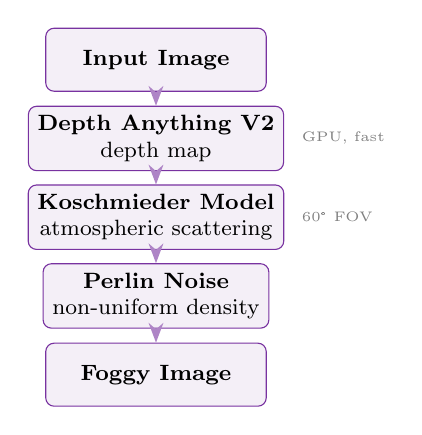
\begin{tikzpicture}
\node[fnode] (in)      at (0,4)   {\textbf{Input Image}};
\node[fnode] (depth)   at (0,3)   {\textbf{Depth Anything V2}\\depth map};
\node[fnode] (kosch)   at (0,2)   {\textbf{Koschmieder Model}\\atmospheric scattering};
\node[fnode] (perlin)  at (0,1)   {\textbf{Perlin Noise}\\non-uniform density};
\node[fnode] (out)     at (0,0)   {\textbf{Foggy Image}};

\draw[farrow] (in) -- (depth);
\draw[farrow] (depth) -- (kosch);
\draw[farrow] (kosch) -- (perlin);
\draw[farrow] (perlin) -- (out);

\node[font=\tiny, text=gray, right=0.1cm of depth] {GPU, fast};
\node[font=\tiny, text=gray, right=0.1cm of kosch] {60\textdegree{} FOV};
\end{tikzpicture}

\vspace{0.5em}
\textbf{Output:} 3$\times$1,001 = \textbf{3,003 images}\\
{\scriptsize (heavy + medium + light, Construction Site)}

\vspace{0.3em}
{\scriptsize Arrow format with \texttt{fog\_label}, \texttt{fog\_visibility} metadata columns.}
\end{column}
\end{columns}
\end{frame}

% ────────────────────────────────────────
\begin{frame}{Day-to-Night Augmentation}
\begin{columns}[T]
\begin{column}{0.55\textwidth}
\textbf{Model:} CycleGAN-Turbo (\texttt{day\_to\_night} checkpoint)

\vspace{0.5em}
\textbf{Pipeline:}
\begin{enumerate}
    \item Load day image $\rightarrow$ resize to $512 \times 512$
    \item Forward pass through CycleGAN-Turbo
    \item Resize output back to original resolution (LANCZOS)
    \item Save night image + copy annotations directly
\end{enumerate}

\vspace{0.5em}
\textbf{Key properties:}
\begin{itemize}
    \item \textbf{1:1 mapping} -- every image gets one night variant
    \item FP16 inference with xformers attention
    \item Annotations \textbf{copied unchanged} (pixel-level transform)
\end{itemize}

\vspace{0.5em}
\textbf{Output:} 3,004 (Construction Site) + 19,846 (SODA)
\end{column}
\begin{column}{0.42\textwidth}
\centering
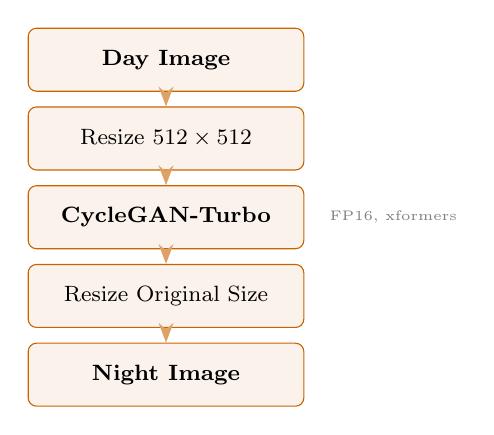
\begin{tikzpicture}
\node[dnode] (in)      at (0,3)   {\textbf{Day Image}};
\node[dnode] (resize1) at (0,2)   {Resize $512\times512$};
\node[dnode] (model)   at (0,1)   {\textbf{CycleGAN-Turbo}};
\node[dnode] (resize2) at (0,0)   {Resize Original Size};
\node[dnode] (out)     at (0,-1)  {\textbf{Night Image}};

\draw[darrow] (in) -- (resize1);
\draw[darrow] (resize1) -- (model);
\draw[darrow] (model) -- (resize2);
\draw[darrow] (resize2) -- (out);

\node[font=\tiny, text=gray, right=0.2cm of model] {FP16, xformers};
\end{tikzpicture}
\end{column}
\end{columns}
\end{frame}

% (Night Weather slide moved above filter section)

% ────────────────────────────────────────
\begin{frame}{Outpainting -- Scale/Distance Augmentation}
\begin{columns}[T]
\begin{column}{0.52\textwidth}
\textbf{Model:} FLUX.1-Fill-dev (bfloat16)

\vspace{0.3em}
\textbf{Idea:} Expand canvas around original image $\rightarrow$ objects appear smaller/more distant.

\vspace{0.3em}
\textbf{Scale factor:} Truncated Gaussian
\[
s \sim \mathcal{N}(\mu{=}0.25,\;\sigma{=}0.05), \quad s \in [0.2, 0.4]
\]
\vspace{-0.5em}
Canvas size: $(1+2s) \times$ original on each axis.

\vspace{0.3em}
\textbf{Bbox transfer:}
\[
x'_1 = \frac{x_1 \cdot W \cdot r + p_x}{W'}, \quad
y'_1 = \frac{y_1 \cdot H \cdot r + p_y}{H'}
\]
\vspace{-0.5em}
{\scriptsize where $r$ = resize factor, $(p_x, p_y)$ = paste offset}

\vspace{0.3em}
\textbf{Prompt:} \textit{``an outdoor construction site with buildings, roads, and open sky in the background''}
\end{column}
\begin{column}{0.45\textwidth}
\centering
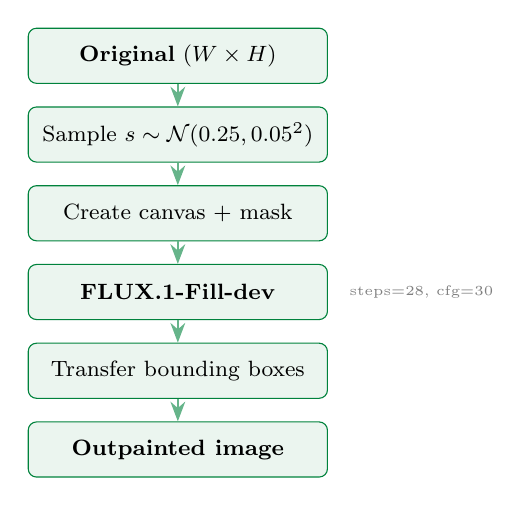
\begin{tikzpicture}
\node[onode] (in)     at (0,4)   {\textbf{Original} ($W \times H$)};
\node[onode] (scale)  at (0,3)   {Sample $s \sim \mathcal{N}(0.25, 0.05^2)$};
\node[onode] (canvas) at (0,2)   {Create canvas + mask};
\node[onode] (flux)   at (0,1)   {\textbf{FLUX.1-Fill-dev}};
\node[onode] (bbox)   at (0,0)   {Transfer bounding boxes};
\node[onode] (out)    at (0,-1)  {\textbf{Outpainted image}};

\draw[oarrow] (in) -- (scale);
\draw[oarrow] (scale) -- (canvas);
\draw[oarrow] (canvas) -- (flux);
\draw[oarrow] (flux) -- (bbox);
\draw[oarrow] (bbox) -- (out);

\node[font=\tiny, text=gray, right=0.15cm of flux] {steps=28, cfg=30};
\end{tikzpicture}

\vspace{0.5em}
\begin{tabular}{lc}
\toprule
\textbf{Dataset} & \textbf{Output} \\
\midrule
Construction Site & 1,323 \\
SODA & 1,001 \\
\bottomrule
\end{tabular}
\end{column}
\end{columns}
\end{frame}

% ════════════════════════════════════════
\section{Benchmarking Framework}
% ════════════════════════════════════════

\begin{frame}{VLM Benchmarking -- Models \& Tasks}
\begin{columns}[T]
\begin{column}{0.45\textwidth}
\textbf{11 Vision-Language Models:}

\vspace{0.3em}
{\small
\begin{tabular}{llc}
\toprule
\textbf{Model} & \textbf{Size} & \textbf{Status} \\
\midrule
InternVL2.5 & 26B & \textcolor{okgreen}{Done} \\
Gemma-3 & 27B & \textcolor{okgreen}{Done} \\
Qwen3-VL & 8B & \textcolor{okgreen}{Done} \\
Phi-4-multimodal & 6B & \textcolor{okgreen}{Done} \\
GPT-4o-mini & API & \textcolor{okgreen}{Done} \\
LLaVA v1.5 & 7B & \textcolor{warnred}{Failed} \\
\midrule
Qwen2.5-VL & 7/32/72B & \textcolor{gray}{Pending} \\
Llama-3.2-Vision & 11B & \textcolor{gray}{Pending} \\
GPT-4o & API & \textcolor{gray}{Pending} \\
\bottomrule
\end{tabular}
}
\end{column}
\begin{column}{0.52\textwidth}
\textbf{4 Benchmark Tasks:}

\vspace{0.3em}
\begin{enumerate}
    \item \textbf{Description} (0-shot captioning)\\
    {\scriptsize Metrics: BERTScore, BLEU, ROUGE-L, METEOR, CLIPScore}

    \vspace{0.2em}
    \item \textbf{VQA Safety} (5-shot, 4 rules)\\
    {\scriptsize Metrics: Per-rule P/R/F1 + bbox IoU}

    \vspace{0.2em}
    \item \textbf{VQA Rule 1} (binary Yes/No)\\
    {\scriptsize PPE compliance detection}

    \vspace{0.2em}
    \item \textbf{Object Detection}\\
    {\scriptsize Normalized bbox, grid-based IoU}
\end{enumerate}

\vspace{0.4em}
{\footnotesize \textbf{Conditions:} original $\times$ weather $\times$ night $\times$ small}
\end{column}
\end{columns}
\end{frame}

% ────────────────────────────────────────
\begin{frame}{Safety Rules for VQA}
\begin{columns}[T]
\begin{column}{0.48\textwidth}
\textbf{\textcolor{warnred}{Rule 1} -- PPE Compliance}
\begin{itemize}
    \item Hard hats, proper clothing, safety shoes
    \item High-vis vests at night
    \item Face shields when cutting/welding
\end{itemize}

\vspace{0.4em}
\textbf{\textcolor{warnred}{Rule 2} -- Safety Harness}
\begin{itemize}
    \item Required at height $\geq$ 3m
    \item Without edge protection
\end{itemize}
\end{column}
\begin{column}{0.48\textwidth}
\textbf{\textcolor{warnred}{Rule 3} -- Edge Protection}
\begin{itemize}
    \item Guardrails, fences required
    \item Underground projects $\geq$ 3m depth
\end{itemize}

\vspace{0.4em}
\textbf{\textcolor{warnred}{Rule 4} -- Excavator Safety}
\begin{itemize}
    \item Workers in blind spots
    \item Within operation radius
\end{itemize}

\vspace{0.6em}
{\footnotesize \textbf{Output format:} JSON with rule ID, reason, bounding box $[x_1, y_1, x_2, y_2]$ in normalized $[0,1]$ space.}
\end{column}
\end{columns}
\end{frame}

% ════════════════════════════════════════
\section{VQA Safety Results}
% ════════════════════════════════════════

\begin{frame}{VQA Safety -- Overall F1 by Model and Condition}
\centering
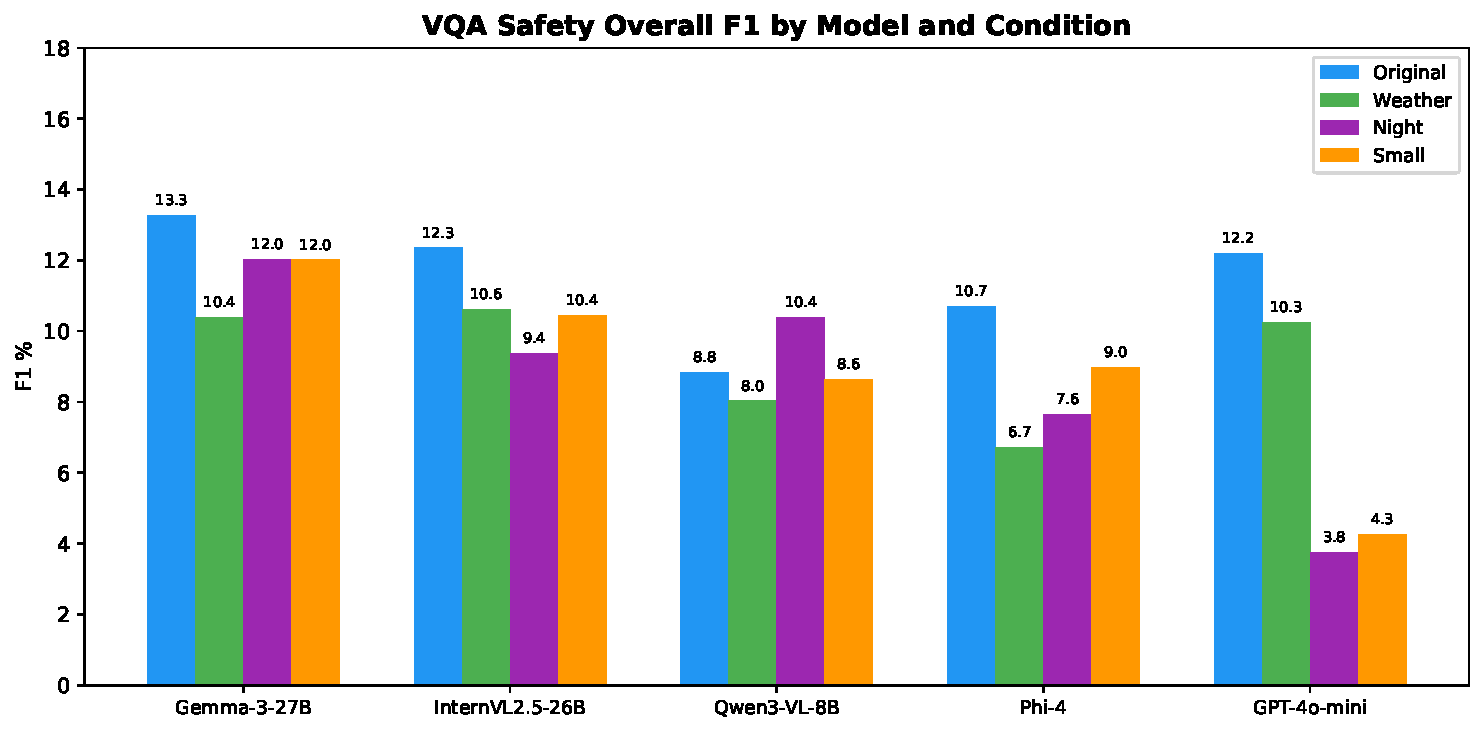
\includegraphics[width=0.92\textwidth]{vqa_f1_bar.pdf}

\vspace{0.3em}
{\scriptsize 5-shot prompting (Phi-4: 2-shot due to memory). LLaVA-1.5-7B omitted (100\% parse errors). Now includes \textbf{Gemma-3-27B}.}
\end{frame}

% ────────────────────────────────────────
\begin{frame}{VQA Safety -- F1 Radar Across Conditions}
\begin{columns}[T]
\begin{column}{0.52\textwidth}
\centering
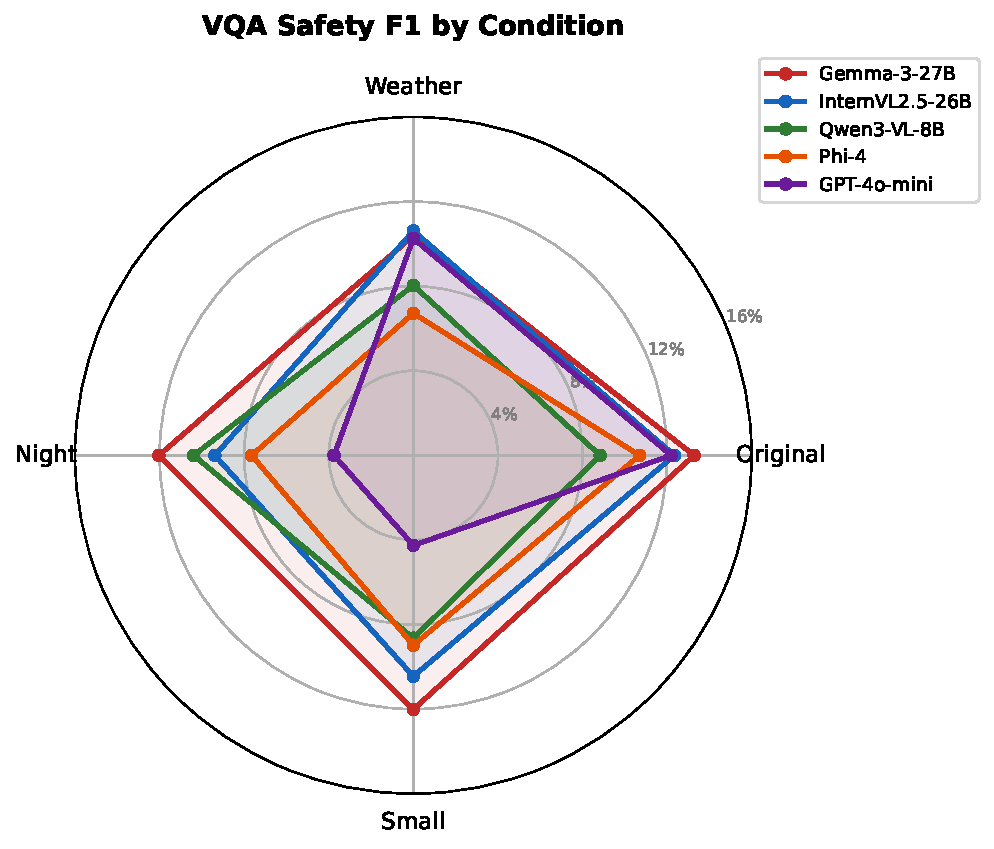
\includegraphics[width=\textwidth]{vqa_f1_radar_conditions.pdf}
\end{column}
\begin{column}{0.45\textwidth}
\centering
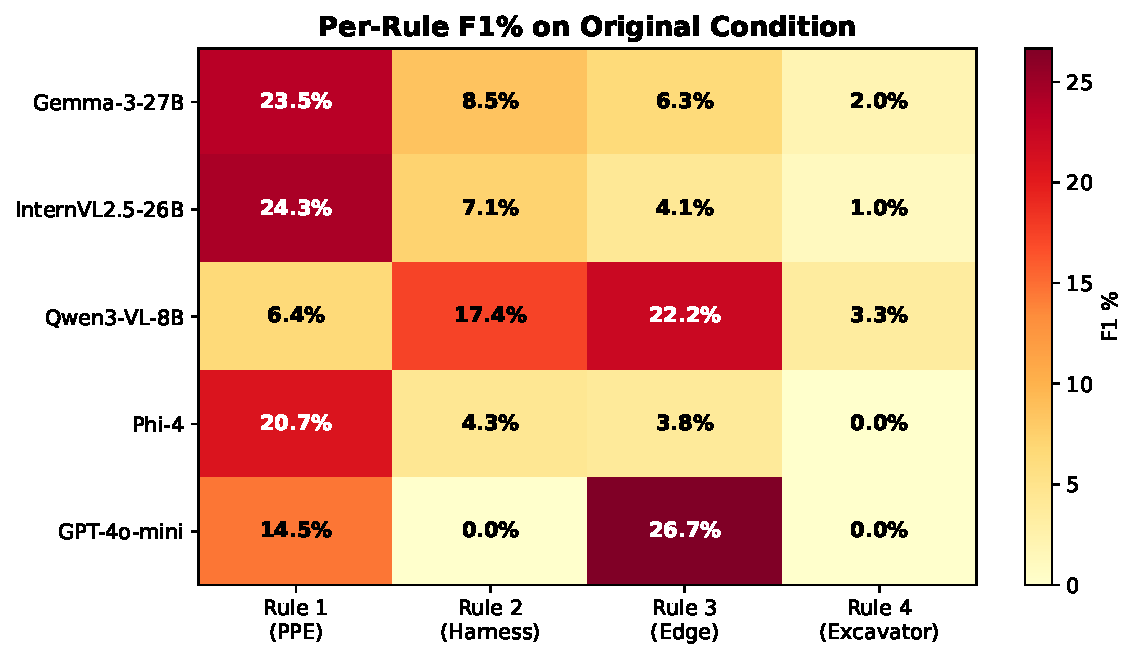
\includegraphics[width=\textwidth]{vqa_per_rule_heatmap.pdf}
\end{column}
\end{columns}
\end{frame}

% ────────────────────────────────────────
\begin{frame}{VQA Safety -- Key Observations}
\begin{columns}[T]
\begin{column}{0.48\textwidth}
\textbf{Model Comparison (6 models evaluated):}
\begin{itemize}
    \item \textbf{Gemma-3-27B}: Best F1 (13.3\%), most robust across conditions (F1 12.0\% on night/small)
    \item \textbf{InternVL2.5-26B}: Very high recall (70--84\%) but extremely low precision (5--7\%) -- over-predicts violations
    \item \textbf{Qwen3-VL-8B}: Best bbox IoU (28.9\%) with balanced P/R -- best localization
    \item \textbf{Phi-4} (2-shot): F1=10.7\%, competitive with GPT-4o-mini; 5-shot OOMs on 1$\times$A100
    \item \textbf{GPT-4o-mini}: $\sim$50\% error rate (model\_error + missing responses)
    \item \textbf{LLaVA-1.5-7B}: 100\% parse errors -- cannot produce JSON
\end{itemize}
\end{column}
\begin{column}{0.48\textwidth}
\textbf{Condition Impact:}
\begin{itemize}
    \item \textcolor{warnred}{Night} degrades GPT-4o-mini most (F1: 12.2$\to$3.8\%)
    \item Gemma-3 and InternVL2.5 are \textbf{robust} across conditions
    \item All models: \textbf{very high false positive rate}
\end{itemize}

\vspace{0.4em}
\textbf{Per-Rule F1\% (original, best model):}

\vspace{0.2em}
{\footnotesize
\begin{tabular}{lcl}
\toprule
\textbf{Rule} & \textbf{Best F1} & \textbf{Best Model} \\
\midrule
R1 (PPE) & 24.3\% & InternVL2.5 \\
R2 (Harness) & 17.4\% & Qwen3-VL \\
R3 (Edge) & 26.7\% & GPT-4o-mini \\
R4 (Excavator) & 12.9\% & Qwen3-VL \\
\bottomrule
\end{tabular}
}

\vspace{0.4em}
{\footnotesize \textbf{Takeaway:} Even the best model achieves $\sim$0.30 IoU. Current VLMs lack domain knowledge for reliable safety inspection.}
\end{column}
\end{columns}
\end{frame}

% ════════════════════════════════════════
\section{Description Task Results}
% ════════════════════════════════════════

\begin{frame}{Description Task -- Model Profiles (Original)}
\begin{columns}[T]
\begin{column}{0.50\textwidth}
\centering
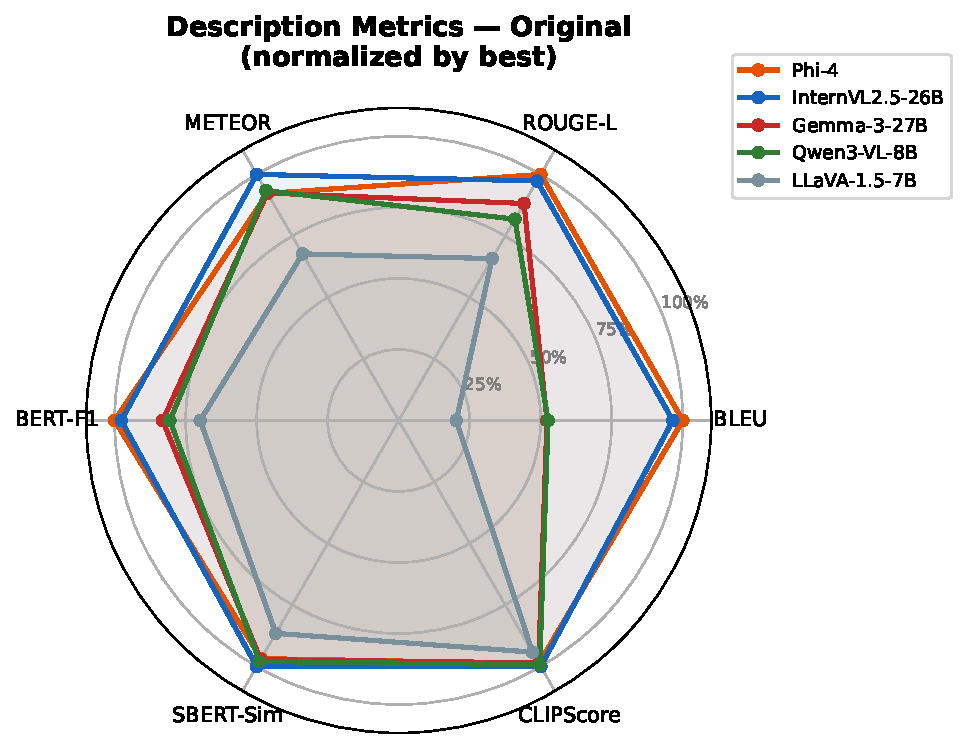
\includegraphics[width=\textwidth]{desc_radar_original.pdf}
\end{column}
\begin{column}{0.46\textwidth}
\vspace{0.5cm}
\textbf{5 models evaluated} (GPT-4o pending):
\begin{itemize}
    \item \textbf{Phi-4} (6B) leads: BLEU 0.065, BERT-F1 0.330 -- \textit{competitive with InternVL 26B}
    \item \textbf{InternVL2.5-26B}: Best ROUGE-L (0.303)
    \item \textbf{Gemma-3-27B}: Between Qwen3 and InternVL
    \item \textbf{CLIPScore} high across all (0.74--0.83) -- descriptions are semantically relevant
    \item \textbf{LLaVA-1.5-7B}: Weakest across all metrics
\end{itemize}

\vspace{0.3em}
{\footnotesize \textbf{Note:} CLIPScore consistently \textit{increases} on night/small conditions (0.80--0.83 vs 0.78 original), likely because augmented images have simpler backgrounds.}
\end{column}
\end{columns}
\end{frame}

% ────────────────────────────────────────
\begin{frame}{Description Task -- All Metrics Heatmap}
\centering
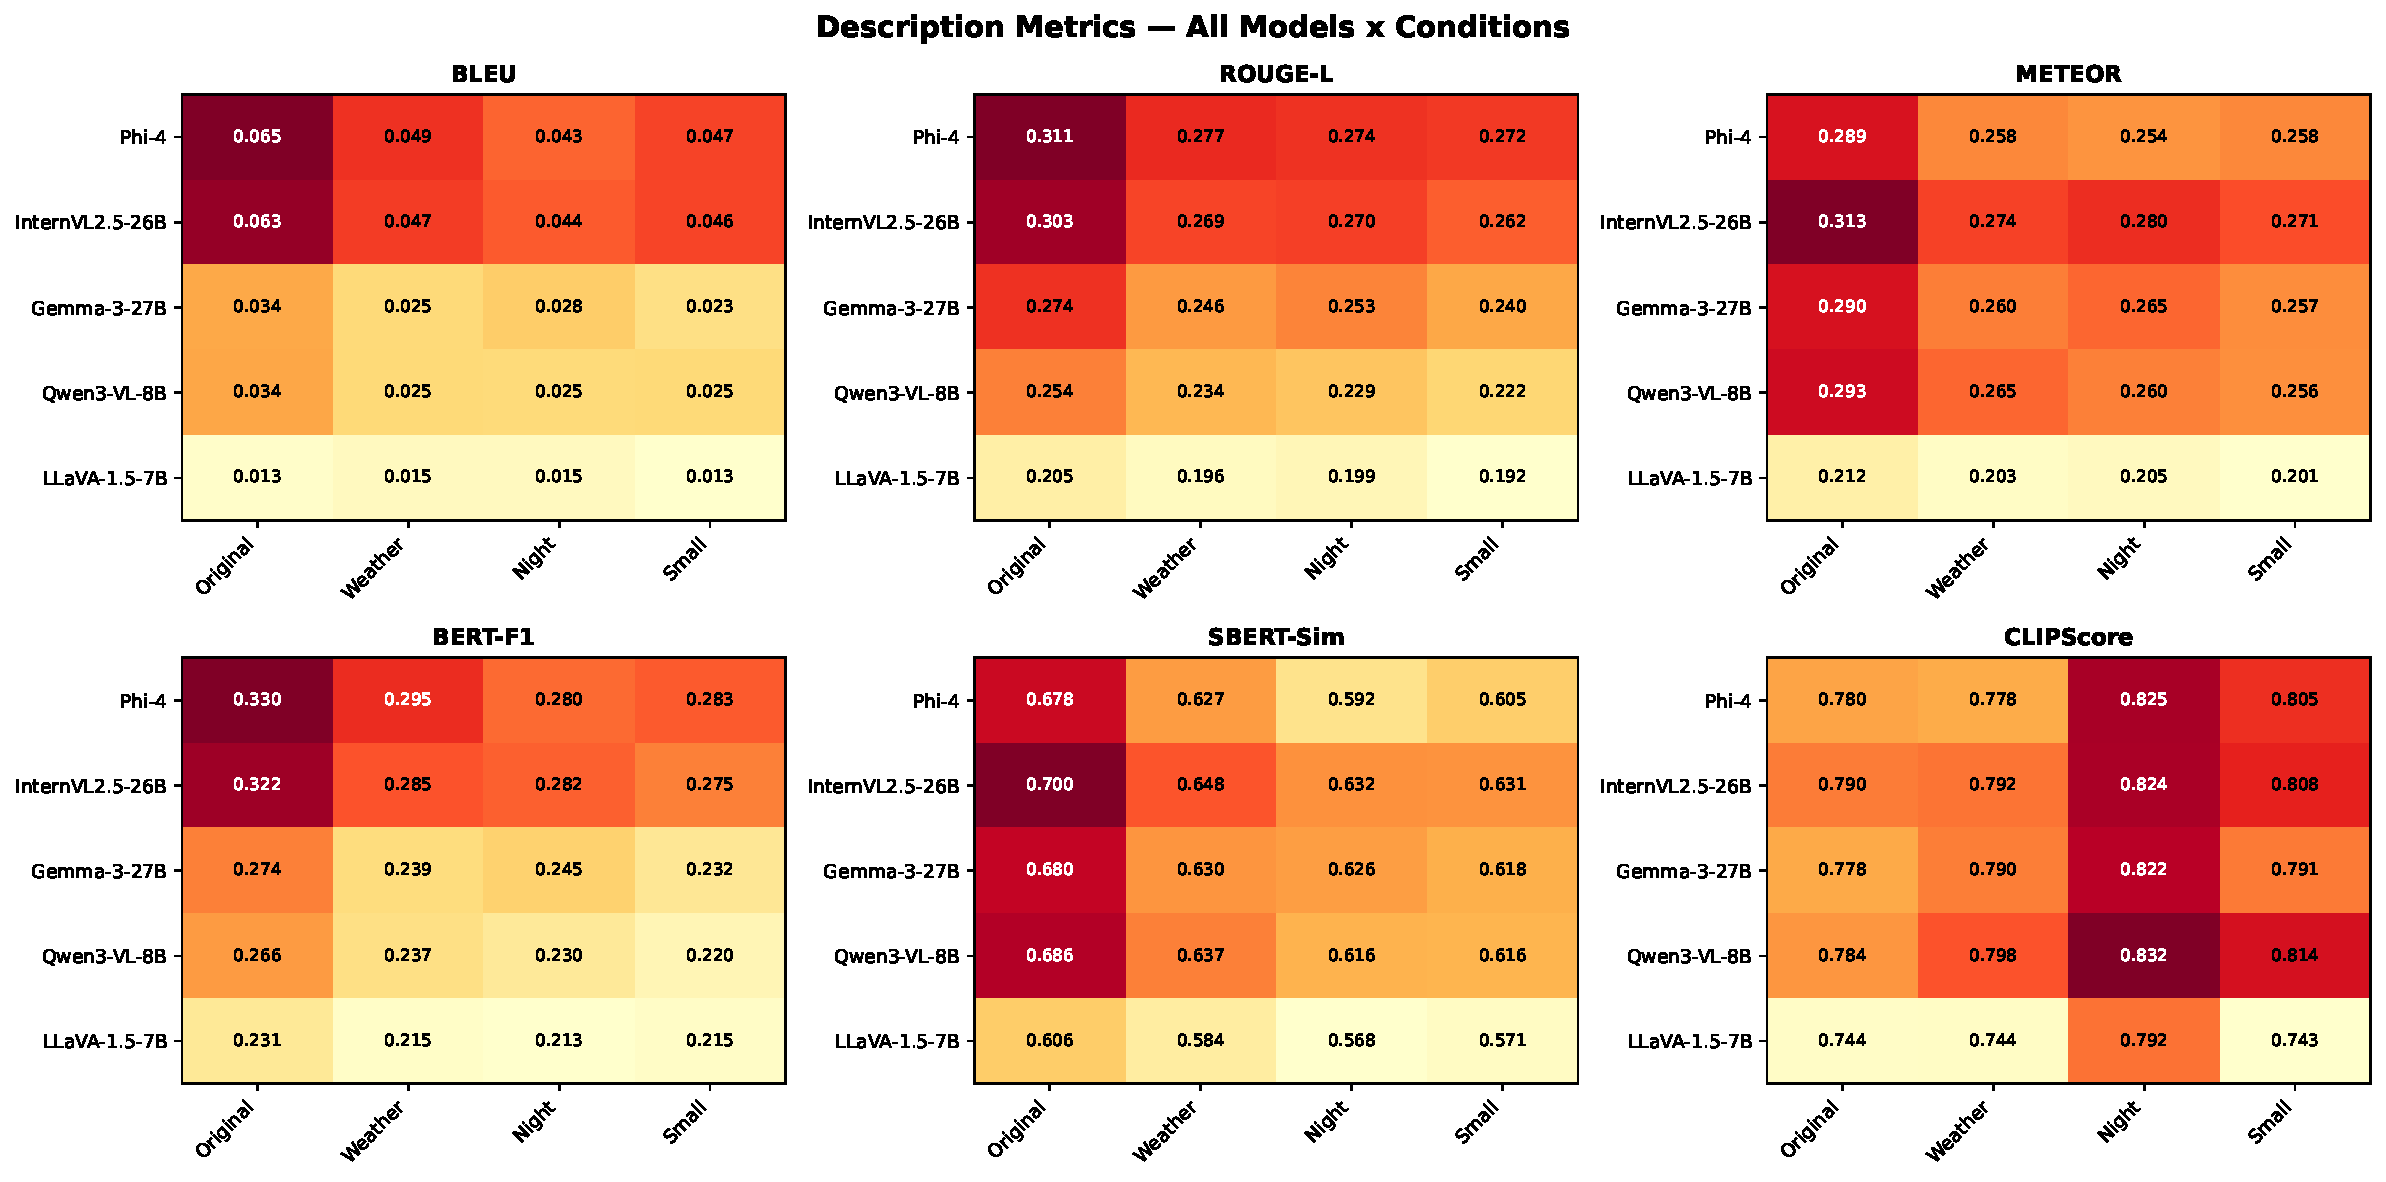
\includegraphics[width=0.88\textwidth]{desc_heatmap.pdf}
\end{frame}

% ────────────────────────────────────────
\begin{frame}{Description Task -- Degradation Under Augmentation}
\centering
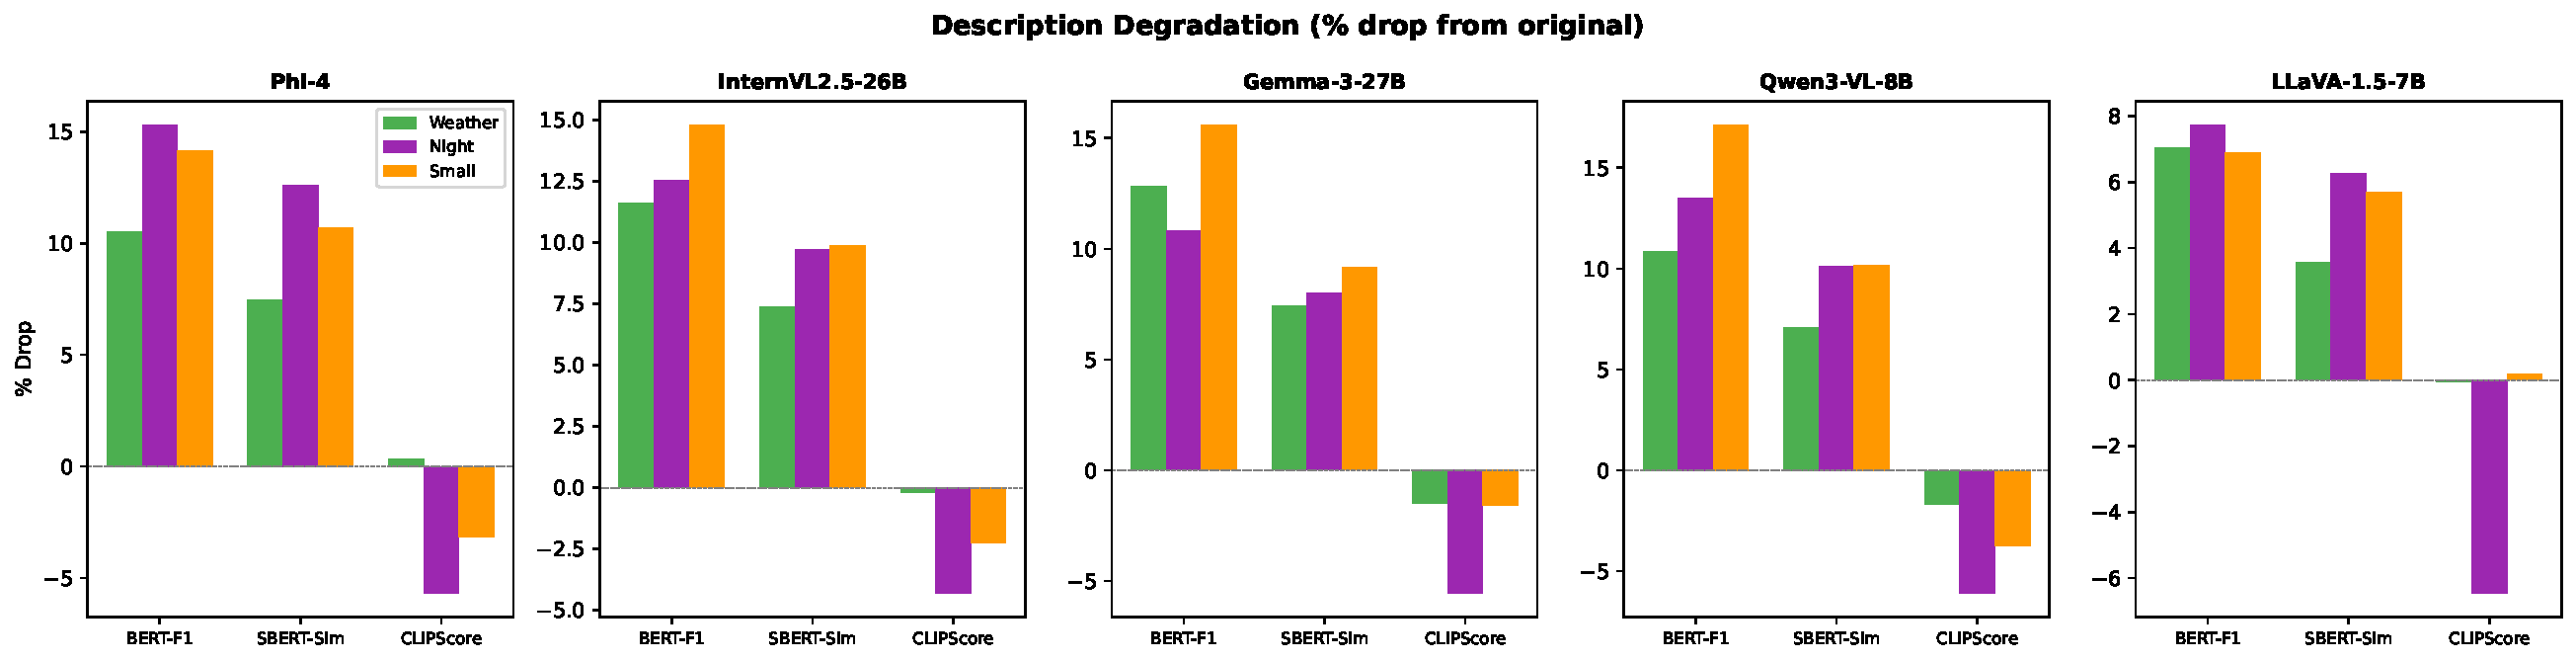
\includegraphics[width=0.95\textwidth]{desc_degradation.pdf}

\vspace{0.3em}
{\scriptsize Positive = performance drop from original. SBERT-Sim and CLIPScore show minimal degradation, confirming augmented images remain semantically consistent.}
\end{frame}

% ════════════════════════════════════════
\section{Augmentation Quality Evaluation}
% ════════════════════════════════════════

\begin{frame}{Augmentation Quality -- FID \& DINO Structure Similarity}
\begin{columns}[T]
\begin{column}{0.48\textwidth}
\textbf{\textcolor{boxblue}{Fr\'{e}chet Inception Distance (FID)}}

\vspace{0.3em}
Measures distributional distance between original and augmented images in Inception-v3 feature space.
\[
\mathrm{FID} = \|\mu_r - \mu_g\|^2 + \mathrm{Tr}\!\left(\Sigma_r + \Sigma_g - 2(\Sigma_r \Sigma_g)^{1/2}\right)
\]

\vspace{0.3em}
\begin{itemize}
    \item \textbf{Lower = closer} to real distribution
    \item Captures both quality and diversity
    \item Computed per augmentation condition
\end{itemize}
\end{column}
\begin{column}{0.48\textwidth}
\textbf{\textcolor{boxorange}{DINO Structure Similarity}}

\vspace{0.3em}
Measures structural preservation using self-supervised DINOv2 features.

\vspace{0.3em}
\begin{itemize}
    \item Extract patch-level features from DINOv2-ViT
    \item Compute cosine similarity between original and augmented feature maps
    \item \textbf{Higher = better} structural preservation
    \item Captures spatial layout, object structure, and scene composition
\end{itemize}

\vspace{0.3em}
{\footnotesize \textbf{Why DINO?} Self-supervised features correlate with human perception of structural similarity better than pixel-level metrics.}
\end{column}
\end{columns}

\vspace{0.6em}
\centering
{\footnotesize \textbf{Goal:} Verify augmented images preserve realism (FID) and scene structure (DINO) while introducing meaningful visual variation.}
\end{frame}

% ────────────────────────────────────────
\begin{frame}{Quality Evaluation -- Per-Condition Analysis}
\begin{columns}[T]
\begin{column}{0.48\textwidth}
\textbf{FID Scores} (lower = closer to original):

\vspace{0.3em}
{\small
\begin{tabular}{lrc}
\toprule
\textbf{Condition} & \textbf{FID $\downarrow$} & \textbf{Images} \\
\midrule
rain\_0          & \textbf{27.8} & 2,211 \\
snow\_0          & 39.6          & 2,159 \\
rain\_2          & 40.8          & 1,208 \\
rain\_1          & 43.6          & 1,243 \\
snow\_2          & 50.5          & 1,796 \\
small            & 60.2          & 1,323 \\
snow\_1          & 69.9          & 1,649 \\
night            & \textcolor{warnred}{97.8} & 3,004 \\
\bottomrule
\end{tabular}
}
\end{column}
\begin{column}{0.48\textwidth}
\textbf{DINO Structural Similarity} (higher = better):

\vspace{0.3em}
{\small
\begin{tabular}{lcc}
\toprule
\textbf{Condition} & \textbf{Mean $\uparrow$} & \textbf{Std} \\
\midrule
rain\_0          & \textbf{0.893} & 0.103 \\
rain\_2          & 0.846          & 0.167 \\
snow\_0          & 0.842          & 0.138 \\
rain\_1          & 0.829          & 0.190 \\
night            & 0.754          & 0.100 \\
snow\_2          & 0.753          & 0.144 \\
snow\_1          & 0.744          & 0.176 \\
small            & \textcolor{warnred}{0.729} & 0.113 \\
\bottomrule
\end{tabular}
}

\vspace{0.3em}
{\scriptsize DINOv2-ViT-S/14, cosine similarity of patch features.}
\end{column}
\end{columns}

\vspace{0.5em}
\textbf{Key Findings:}
\begin{itemize}
    \item \textbf{Rain\_0} best quality: lowest FID (27.8) and highest DINO (0.893) -- subtle, realistic effect
    \item \textbf{Night} largest distribution shift (FID 97.8) but decent structure preservation (DINO 0.754)
    \item \textbf{Small} (outpainting) lowest structural similarity (0.729) -- expected due to scene expansion
    \item Snow styles show more variation than rain (FID 39.6--69.9 vs 27.8--43.6)
\end{itemize}
\end{frame}

% ════════════════════════════════════════
\section{Project Architecture}
% ════════════════════════════════════════

\begin{frame}{Repository Structure}
\centering
\resizebox{0.95\textwidth}{!}{%
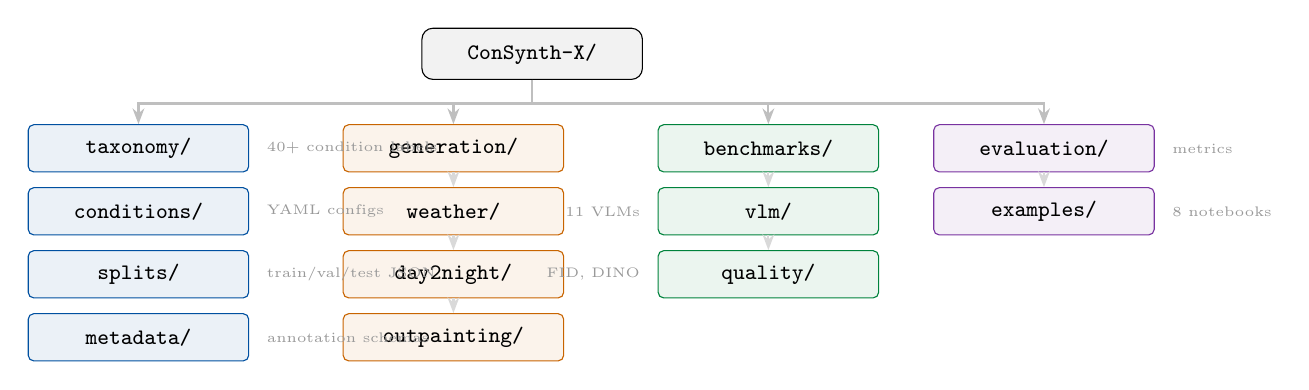
\begin{tikzpicture}

\node[rroot] (r) at (0,0) {ConSynth-X/};

% Left side - data
\node[rdir=boxblue]   (tax) at (-5, -1.2) {taxonomy/};
\node[rdir=boxblue]   (con) at (-5, -2.0) {conditions/};
\node[rdir=boxblue]   (spl) at (-5, -2.8) {splits/};
\node[rdir=boxblue]   (met) at (-5, -3.6) {metadata/};

% Center - generation
\node[rdir=boxorange] (gen) at (-1, -1.2) {generation/};
\node[rdir=boxorange] (gw) at (-1, -2.0) {weather/};
\node[rdir=boxorange] (gd) at (-1, -2.8) {day2night/};
\node[rdir=boxorange] (go) at (-1, -3.6) {outpainting/};

% Right side - benchmarks
\node[rdir=boxgreen]  (ben) at (3, -1.2) {benchmarks/};
\node[rdir=boxgreen]  (bv) at (3, -2.0) {vlm/};
\node[rdir=boxgreen]  (bd) at (3, -2.8) {quality/};

% Far right - eval & examples
\node[rdir=boxpurple] (eva) at (6.5, -1.2) {evaluation/};
\node[rdir=boxpurple] (exa) at (6.5, -2.0) {examples/};

% Arrows from root
\draw[rarrow] (r.south) -- ++(0,-0.3) -| (tax.north);
\draw[rarrow] (r.south) -- ++(0,-0.3) -| (gen.north);
\draw[rarrow] (r.south) -- ++(0,-0.3) -| (ben.north);
\draw[rarrow] (r.south) -- ++(0,-0.3) -| (eva.north);

% Sub-arrows
\draw[rarrow, gray!30] (gen.south) -- (gw.north);
\draw[rarrow, gray!30] (gw.south) -- (gd.north);
\draw[rarrow, gray!30] (gd.south) -- (go.north);
\draw[rarrow, gray!30] (ben.south) -- (bv.north);
\draw[rarrow, gray!30] (bv.south) -- (bd.north);
\draw[rarrow, gray!30] (eva.south) -- (exa.north);

% Descriptions
\node[rdesc, right=0.1cm of tax] {40+ condition labels};
\node[rdesc, right=0.1cm of con] {YAML configs};
\node[rdesc, right=0.1cm of spl] {train/val/test JSON};
\node[rdesc, right=0.1cm of met] {annotation schemas};
\node[rdesc, left=0.1cm of bv]  {11 VLMs};
\node[rdesc, left=0.1cm of bd]  {FID, DINO};
\node[rdesc, right=0.1cm of eva] {metrics};
\node[rdesc, right=0.1cm of exa] {8 notebooks};
\end{tikzpicture}}%
\end{frame}

% ════════════════════════════════════════
\section{Downstream Detection -- Sensitivity Analysis}
% ════════════════════════════════════════

\begin{frame}{SSIM/LPIPS Threshold Sensitivity -- Experimental Design}
\begin{columns}[T]
\begin{column}{0.48\textwidth}
\textbf{Goal:} Determine optimal SSIM/LPIPS thresholds for quality filtering of synthetic augmentation data.

\vspace{0.3em}
\textbf{Pipeline:}
\begin{enumerate}
    \item Generate rain/snow via IP2P + physics overlay
    \item Filter by SSIM $\in [\tau, 0.95]$ and LPIPS $< \lambda$
    \item Combine filtered augmented + original data
    \item Train YOLOv8n (20 epochs, seed=42)
    \item Evaluate mAP@0.5 on held-out test set
\end{enumerate}

\vspace{0.3em}
\textbf{Training setup:}
\begin{itemize}
    \item Model: YOLOv8n, imgsz=640, batch=16
    \item 3 classes: excavator, rebar, worker
    \item Val: 1,000 images from test split
\end{itemize}
\end{column}
\begin{column}{0.48\textwidth}
\textbf{7 threshold configurations:}

\vspace{0.3em}
{\small
\begin{tabular}{lccc}
\toprule
\textbf{Config} & \textbf{SSIM$_r$} & \textbf{SSIM$_s$} & \textbf{LPIPS} \\
\midrule
baseline  & --    & --    & --   \\
loose     & 0.40  & 0.40  & 0.50 \\
moderate  & 0.50  & 0.50  & 0.40 \\
current   & 0.60  & 0.50  & 0.35 \\
strict    & 0.65  & 0.60  & 0.30 \\
tight     & 0.70  & 0.65  & 0.25 \\
no\_lpips & 0.60  & 0.50  & --   \\
\bottomrule
\end{tabular}
}

\vspace{0.3em}
{\scriptsize $r$ = rain, $s$ = snow. Baseline uses original data only (no augmentation).}
\end{column}
\end{columns}
\end{frame}

% ────────────────────────────────────────
\begin{frame}{Sensitivity Results -- YOLOv8n Detection Performance}
\centering
{\small
\begin{tabular}{l c c c c c c}
\toprule
\textbf{Config} & \textbf{Train} & \textbf{mAP@0.5} & \textbf{mAP@.5:.95} & \textbf{Prec.} & \textbf{Recall} & \textbf{Excavator} \\
\midrule
baseline          & 7,009  & \textbf{0.562} & 0.338 & \textbf{0.674} & 0.558 & 0.906 \\
\rowcolor{lightred}
loose$^\dagger$   & 17,391 & 0.535 & 0.344 & 0.589 & 0.579 & 0.920 \\
\rowcolor{lightred}
moderate$^\dagger$ & 17,391 & 0.535 & 0.344 & 0.589 & 0.579 & 0.920 \\
current           & 17,390 & 0.547 & 0.339 & 0.617 & 0.558 & 0.916 \\
strict            & 16,379 & 0.538 & \textbf{0.349} & 0.583 & \textbf{0.580} & 0.915 \\
tight             & 14,948 & 0.542 & 0.344 & 0.613 & 0.576 & 0.909 \\
\rowcolor{lightred}
no\_lpips$^\dagger$ & 17,391 & 0.535 & 0.344 & 0.589 & 0.579 & 0.920 \\
\bottomrule
\end{tabular}
}

\vspace{0.4em}
{\scriptsize $^\dagger$ \textcolor{warnred}{\textbf{Identical results}} -- see next slide for explanation.}

\vspace{0.3em}
\textbf{Per-class AP@0.5:}
{\scriptsize Excavator consistently high (0.91+). Rebar struggles (0.19--0.26). Worker stable (0.45--0.52).}
\end{frame}

% ────────────────────────────────────────
\begin{frame}{Sensitivity Analysis -- Limitations Found}
\begin{columns}[T]
\begin{column}{0.48\textwidth}
\textbf{\textcolor{warnred}{Problem: Pre-filtered Arrow data}}

The Arrow batch files used for training contain \textbf{only images that already passed} the \texttt{current} threshold (SSIM$\geq$0.60 rain, $\geq$0.50 snow).

\vspace{0.3em}
\textbf{Consequence:}
\begin{itemize}
    \item Looser thresholds (loose, moderate) cannot recover dropped images
    \item \texttt{no\_lpips} produces identical data to \texttt{loose} (LPIPS filter was already applied)
    \item Only \texttt{strict} and \texttt{tight} actually filter differently
\end{itemize}

\vspace{0.3em}
\textbf{Evidence:}
{\scriptsize
\begin{tabular}{lcc}
\toprule
\textbf{Config} & \textbf{Rain} & \textbf{Snow} \\
\midrule
loose/mod/no\_lpips & 3,627 & 6,755 \\
current & 3,626 & 6,755 \\
strict & 3,048 & 6,322 \\
tight & 2,259 & 5,680 \\
\bottomrule
\end{tabular}
}
\end{column}
\begin{column}{0.48\textwidth}
\textbf{\textcolor{warnred}{Additional issues:}}

\begin{enumerate}
    \item \textbf{Snow has no LPIPS scores} -- LPIPS was never computed for snow diffusion, making \texttt{no\_lpips} config meaningless (65\% of augmented data)

    \item \textbf{Val set is clean images only} -- baseline outperforms all augmented configs because the test set has no weather conditions

    \item \textbf{Only 20 epochs} -- may not be sufficient for convergence with larger datasets (17k vs 7k)
\end{enumerate}

\vspace{0.3em}
\textbf{\textcolor{okgreen}{Fix plan:}}
\begin{itemize}
    \item Re-run filtering from raw meta CSVs + \textbf{unfiltered} Arrow batches
    \item Compute LPIPS for snow
    \item Add weather-augmented val set
    \item Increase to 50 epochs
\end{itemize}
\end{column}
\end{columns}
\end{frame}

% ════════════════════════════════════════
\section{Current Status \& Next Steps}
% ════════════════════════════════════════

\begin{frame}{Current Status \& Next Steps}
\begin{columns}[T]
\begin{column}{0.48\textwidth}
\textbf{\textcolor{okgreen}{Completed:}}
\begin{itemize}
    \item[\textcolor{okgreen}{$\checkmark$}] 5 augmentation pipelines total
    \item[\textcolor{okgreen}{$\checkmark$}] VLM benchmark framework (11 models)
    \item[\textcolor{okgreen}{$\checkmark$}] VQA Safety: 6 models $\times$ 4 conditions
    \item[\textcolor{okgreen}{$\checkmark$}] Description: 5 models $\times$ 4 conditions
    \item[\textcolor{okgreen}{$\checkmark$}] Augmentation quality (FID, DINO)
    \item[\textcolor{okgreen}{$\checkmark$}] Gemma-3-27B, Phi-4 integrated
    \item[\textcolor{okgreen}{$\checkmark$}] Fog pipeline (Koschmieder + DA V2)
    \item[\textcolor{okgreen}{$\checkmark$}] Diffusion rain/snow (IP2P, 10,382 images)
    \item[\textcolor{okgreen}{$\checkmark$}] SODA day-to-night (19,846 images)
    \item[\textcolor{okgreen}{$\checkmark$}] Sensitivity analysis v1 (7 configs, YOLOv8n)
\end{itemize}
\end{column}
\begin{column}{0.48\textwidth}
\textbf{\textcolor{infobl}{In Progress / Next:}}
\begin{itemize}
    \item[\textcolor{warnred}{$\circ$}] \textbf{Fix sensitivity:} re-run from unfiltered Arrow data (current results invalid for loose/moderate)
    \item[\textcolor{warnred}{$\circ$}] Compute LPIPS for snow diffusion
    \item[\textcolor{warnred}{$\circ$}] Add weather-augmented val set
    \item[\textcolor{infobl}{$\circ$}] Re-train with 50 epochs
    \item[\textcolor{infobl}{$\circ$}] Run remaining VLMs (Qwen2.5, Llama-3.2, GPT-4o)
    \item[\textcolor{infobl}{$\circ$}] FID \& DINO eval on fog + diffusion weather
\end{itemize}

\vspace{0.3em}
\textbf{\textcolor{gray}{Planned:}}
\begin{itemize}
    \item[\textcolor{gray}{$\circ$}] Per-condition robustness metrics (AP)
    \item[\textcolor{gray}{$\circ$}] Failure-case visualizations
    \item[\textcolor{gray}{$\circ$}] Paper with reporting tables
\end{itemize}
\end{column}
\end{columns}
\end{frame}

% ════════════════════════════════════════
\begin{frame}{}
\centering
\vspace{2cm}
{\Huge\bfseries Thank You}

\vspace{1cm}
{\large Questions?}

\vspace{1cm}
{\footnotesize
Repository: \texttt{ConSynth-X/}\\
Viet Huy Duong -- \texttt{vduong1@kent.edu}\\
Kent State University
}
\end{frame}

\end{document}
